%
%  PARA TRABALLOS EN GALLEGO USAR (LINEA 12): \usepackage[galician]{babel}
%  PARA TRABALLOS EN CASTELLANO USAR (LINEA 13): \usepackage[spanish]{babel}
%
% Para los acentos usamos codificacion UTF-8 (LINEA 10): \usepackage[utf8]{inputenc} 
% Si se usase la codificacion es_ES.ISO-8859-1 (LINEA 11): \usepackage[latin1]{inputenc}
% La conversion de acentos se hace con: iconv -f UTF-8 -t ISO-8859-1 filename.tex
%
% Como se incluyen figuras eps hay que compilar con: latex traballo , dvipdf traballo
%

\documentclass[12pt,twoside,a4paper]{book}
% pódense engadir todos os packages necesarios
\usepackage[utf8]{inputenc}
% \usepackage[latin1]{inputenc}
% \usepackage[galician]{babel}
\usepackage[spanish]{babel}
\usepackage{graphicx}
\usepackage[dvips]{epsfig}
\usepackage{amssymb}
\usepackage{eurosym}
\usepackage{float}
\usepackage{latexsym}
\usepackage{a4}
\usepackage{listings}
% \usepackage{hyperref} % menús no pdf pero non leva ben co package galician

\usepackage{tabularx}
\usepackage{xkeyval}

% TABLA TAREA EDT

% define the key (arguments)
\makeatletter
\define@key{wpkeys}{id}{%
  \def\wpid{#1}
}
\define@key{wpkeys}{name}{%
  \def\wpname{#1}
}
\define@key{wpkeys}{duration}{%
  \def\wpduration{#1 días}
}
\define@key{wpkeys}{results}{%
  \def\wpresults{#1}
}
\makeatother
% end of key definition

% new command
\newcommand{\WorkItem}[2][]{%
    \setkeys{wpkeys}{#1}%
    \vspace{5mm}
    \begin{tabularx}{\linewidth}{|p{3cm}|X|}
        \hline
        \textbf{Id} & \wpid \tabularnewline
        \hline
        \textbf{Tarea} & \wpname \tabularnewline
        \hline
        \textbf{Duración} & \wpduration \tabularnewline
        \hline
        \textbf{Descripción} & #2 \tabularnewline
        \hline
        \textbf{Salida} & \wpresults \tabularnewline
        \hline
    \end{tabularx}
}
% end of command definition

% TABLA REQUISITO

% define the key (arguments)
\makeatletter
\define@key{rqkeys}{id}{%
  \def\rqid{#1}
}
\define@key{rqkeys}{name}{%
  \def\rqname{#1}
}
\define@key{rqkeys}{description}{%
  \def\rqdescription{#1}
}
\define@key{rqkeys}{priority}{%
  \def\rqpriority{#1}
}
\makeatother
% end of key definition

% new command
\newcommand{\Req}[2][]{%
    \setkeys{rqkeys}{#1}%
    \vspace{5mm}
    \begin{tabularx}{\linewidth}{|p{3cm}|X|}
        \hline
        \textbf{\rqid} & \rqname \tabularnewline
        \hline
        \textbf{Descripción} & \rqdescription \tabularnewline
        \hline
        \textbf{Importancia} & \rqpriority \tabularnewline
        \hline
    \end{tabularx}
}
% end of command definition


\begin{document}
\pagestyle{empty}
\begin{center}
{\bf\Large UNIVERSIDAD DE SANTIAGO DE COMPOSTELA}

\vspace{0.5cm}

\includegraphics[width=5cm]{figuras/logo_usc.eps}

\vspace{0.5cm}
{\bf\large ESCUELA TÉCNICA SUPERIOR DE INGENIERÍA}

\vspace{2cm}
{\bf\LARGE Paralelización del algoritmo Progressive Hedging para la resolución de problemas estocásticos}
\end{center} 

\vspace{2cm}
\hspace{4cm}\begin{tabular}{l}
{\it\Large Autor:} \\
{\bf\Large Cristofer Canosa Domínguez} \\
~ \\
{\it\Large Directores:} \\
{\bf\Large Juan Carlos Pichel Campos} \\
{\bf\Large Diego Rodríguez Martínez} \\
\end{tabular}

\vspace{2cm}
\begin{center}
{\bf\Large Grado en Ingeniería Informática}

\vspace{0.5cm}
{\bf\large Julio 2018}

\vspace{0.5cm}
Trabajo de Fin de Grado presentado en la Escuela Técnica Superior de Ingeniería de la Universidad de Santiago de Compostela para la obtención del Grado en Ingeniería Informática
\end{center}


\cleardoublepage
\pagestyle{plain}
\pagenumbering{roman}

\includegraphics[width=4cm]{figuras/logo_usc.eps}

\vspace{1cm}
{\bf D. (Juan Carlos Pichel Campos)}, Profesor do Departamento de Electrónica e Computación da Universidade de Santiago de Compostela, e {\bf D. (Diego Rodríguez Martínez)}, Profesor do Departamento de Electrónica e Computación da Universidade de Santiago de Compostela,

\vspace{1cm}
INFORMAN:

\vspace{1cm}
Que la presente memoria, titulada {\it (Paralelización del algoritmo Progressive Hedging para la resolución de problemas estocásticos)}, presentada por {\bf D. (Cristofer Canosa Domínguez)} para superar los créditos correspondientes al Trabajo de Fin de Grado de la titulación de Grado en Ingeniería Informática, se realizó bajo nuestra dirección en el Departamento de Electrónica y Computación de la Universidad de Santiago de Compostela.

\vspace{1cm}
Y para que así conste a los efectos oportunos, expiden el presente informe en Santiago de Compostela a 26 de Julio de 2018:

\vspace{2cm}
\begin{tabular}{lll}
El director, & El codirector, & El alumno, \\
~ \\
~ \\
~ \\
~ \\
~ \\
~ \\
~ \\
(Juan Carlos Pichel Campos) & (Diego Rodríguez Martínez) & (Cristofer Canosa Domínguez)
\end{tabular}

 % paxina de certificación (optativa)
\cleardoublepage
\pagestyle{plain}
\chapter*{Agradecementos}
Se se quere pór algún agradecemento, este vai aquí.

 % paxina de agradecementos (optativa) 
\cleardoublepage
\pagestyle{plain}
\chapter*{Resumo}

La paralelización de un código busca adaptar la ejecución secuencial de forma que se ejecuten varias instrucciones al mismo tiempo. Esto no solo reduce el tiempo de ejecución si no que permite abordar problemas de mayor tamaño y aprovechar clústeres de computación con múltiples nodos. De esta forma el código se puede escalar más fácilmente y asignar un mayor número de recursos a su ejecución.\\

En este proyecto estudiaremos el módulo de resolución de problemas estocásticos de Pyomo y buscaremos herramientas que nos permitan adaptar el algoritmo existente a una ejecución paralela. Una vez diseñado e implementado el nuevo módulo se realizarán una serie de pruebas que concluirán en un informe de rendimiento del nuevo algoritmo.\\

El resultado final será una nueva implementación paralela para la resolución de problemas estocásticos como parte de Pyomo. % páxina de resumo (optativa) 

\cleardoublepage
\pagestyle{plain}
\tableofcontents
\listoffigures
\listoftables

% Agora incluimos os capítulos. Cambiamos a numeración e as cabeceiras
\cleardoublepage
\pagenumbering{arabic}
\setcounter{page}{1}
\pagestyle{headings}
\chapter{Introdución}

Este proyecto nace con la intención de trabajar sobre el proyecto de código abierto Pyomo, y aportar una implementación paralela de su módulo de resolución de problemas mediante programación estocástica. Con esto buscamos que este programa pueda resolver problemas de mayor tamaño en un tiempo razonable aprovechando el uso de computación distribuida.

\section{Pyomo y la Programación Estocástica}

% Explicar el proyecto Pyomo, que resuelve muchos tipos de problemas. Ver la motivación original del proyecto. 
% Programación Estocástica, tipos de problemas y aplicación en el mundo real.

Pyomo \cite{pyomo} es un paquete de software basado en Python destinado a la formulación y solución de modelos de optimización. Fue desarrollado por \textit{Sandia National Laboratories} y \textit{University of California, Davis} y permite la solución de multitud de problemas distintos, permitiendo su utilización con multitud de solvers de terceros como CPLEX o GLPK. Pyomo es un proyecto extensible mediante la integración de plugins que pueden ser programados por la comunidad para uso privado o público gracias a su filosofía de código abierto.\\

En este proyecto se ampliará el módulo PySP, el paquete de Pyomo dedicado a la solución de problemas estocásticos. La Programación Estocástica \cite{stochasticProgramming} resuelve problemas de optimización donde existe un cierto grado de incertidumbre. Esta incertidumbre hace que no podamos pensar en un problema como algo estático. Los distintos valores posibles generarán escenarios diferentes y, si contamos con varias variables inciertas y dependencias entre ellas, podemos tener un problema que se desarrolle en más de una fase. Por esto, este tipo de problemas suelen representarse como un árbol donde cada nodo es un posible escenario.\\

\begin{figure}[H]
    \centerline{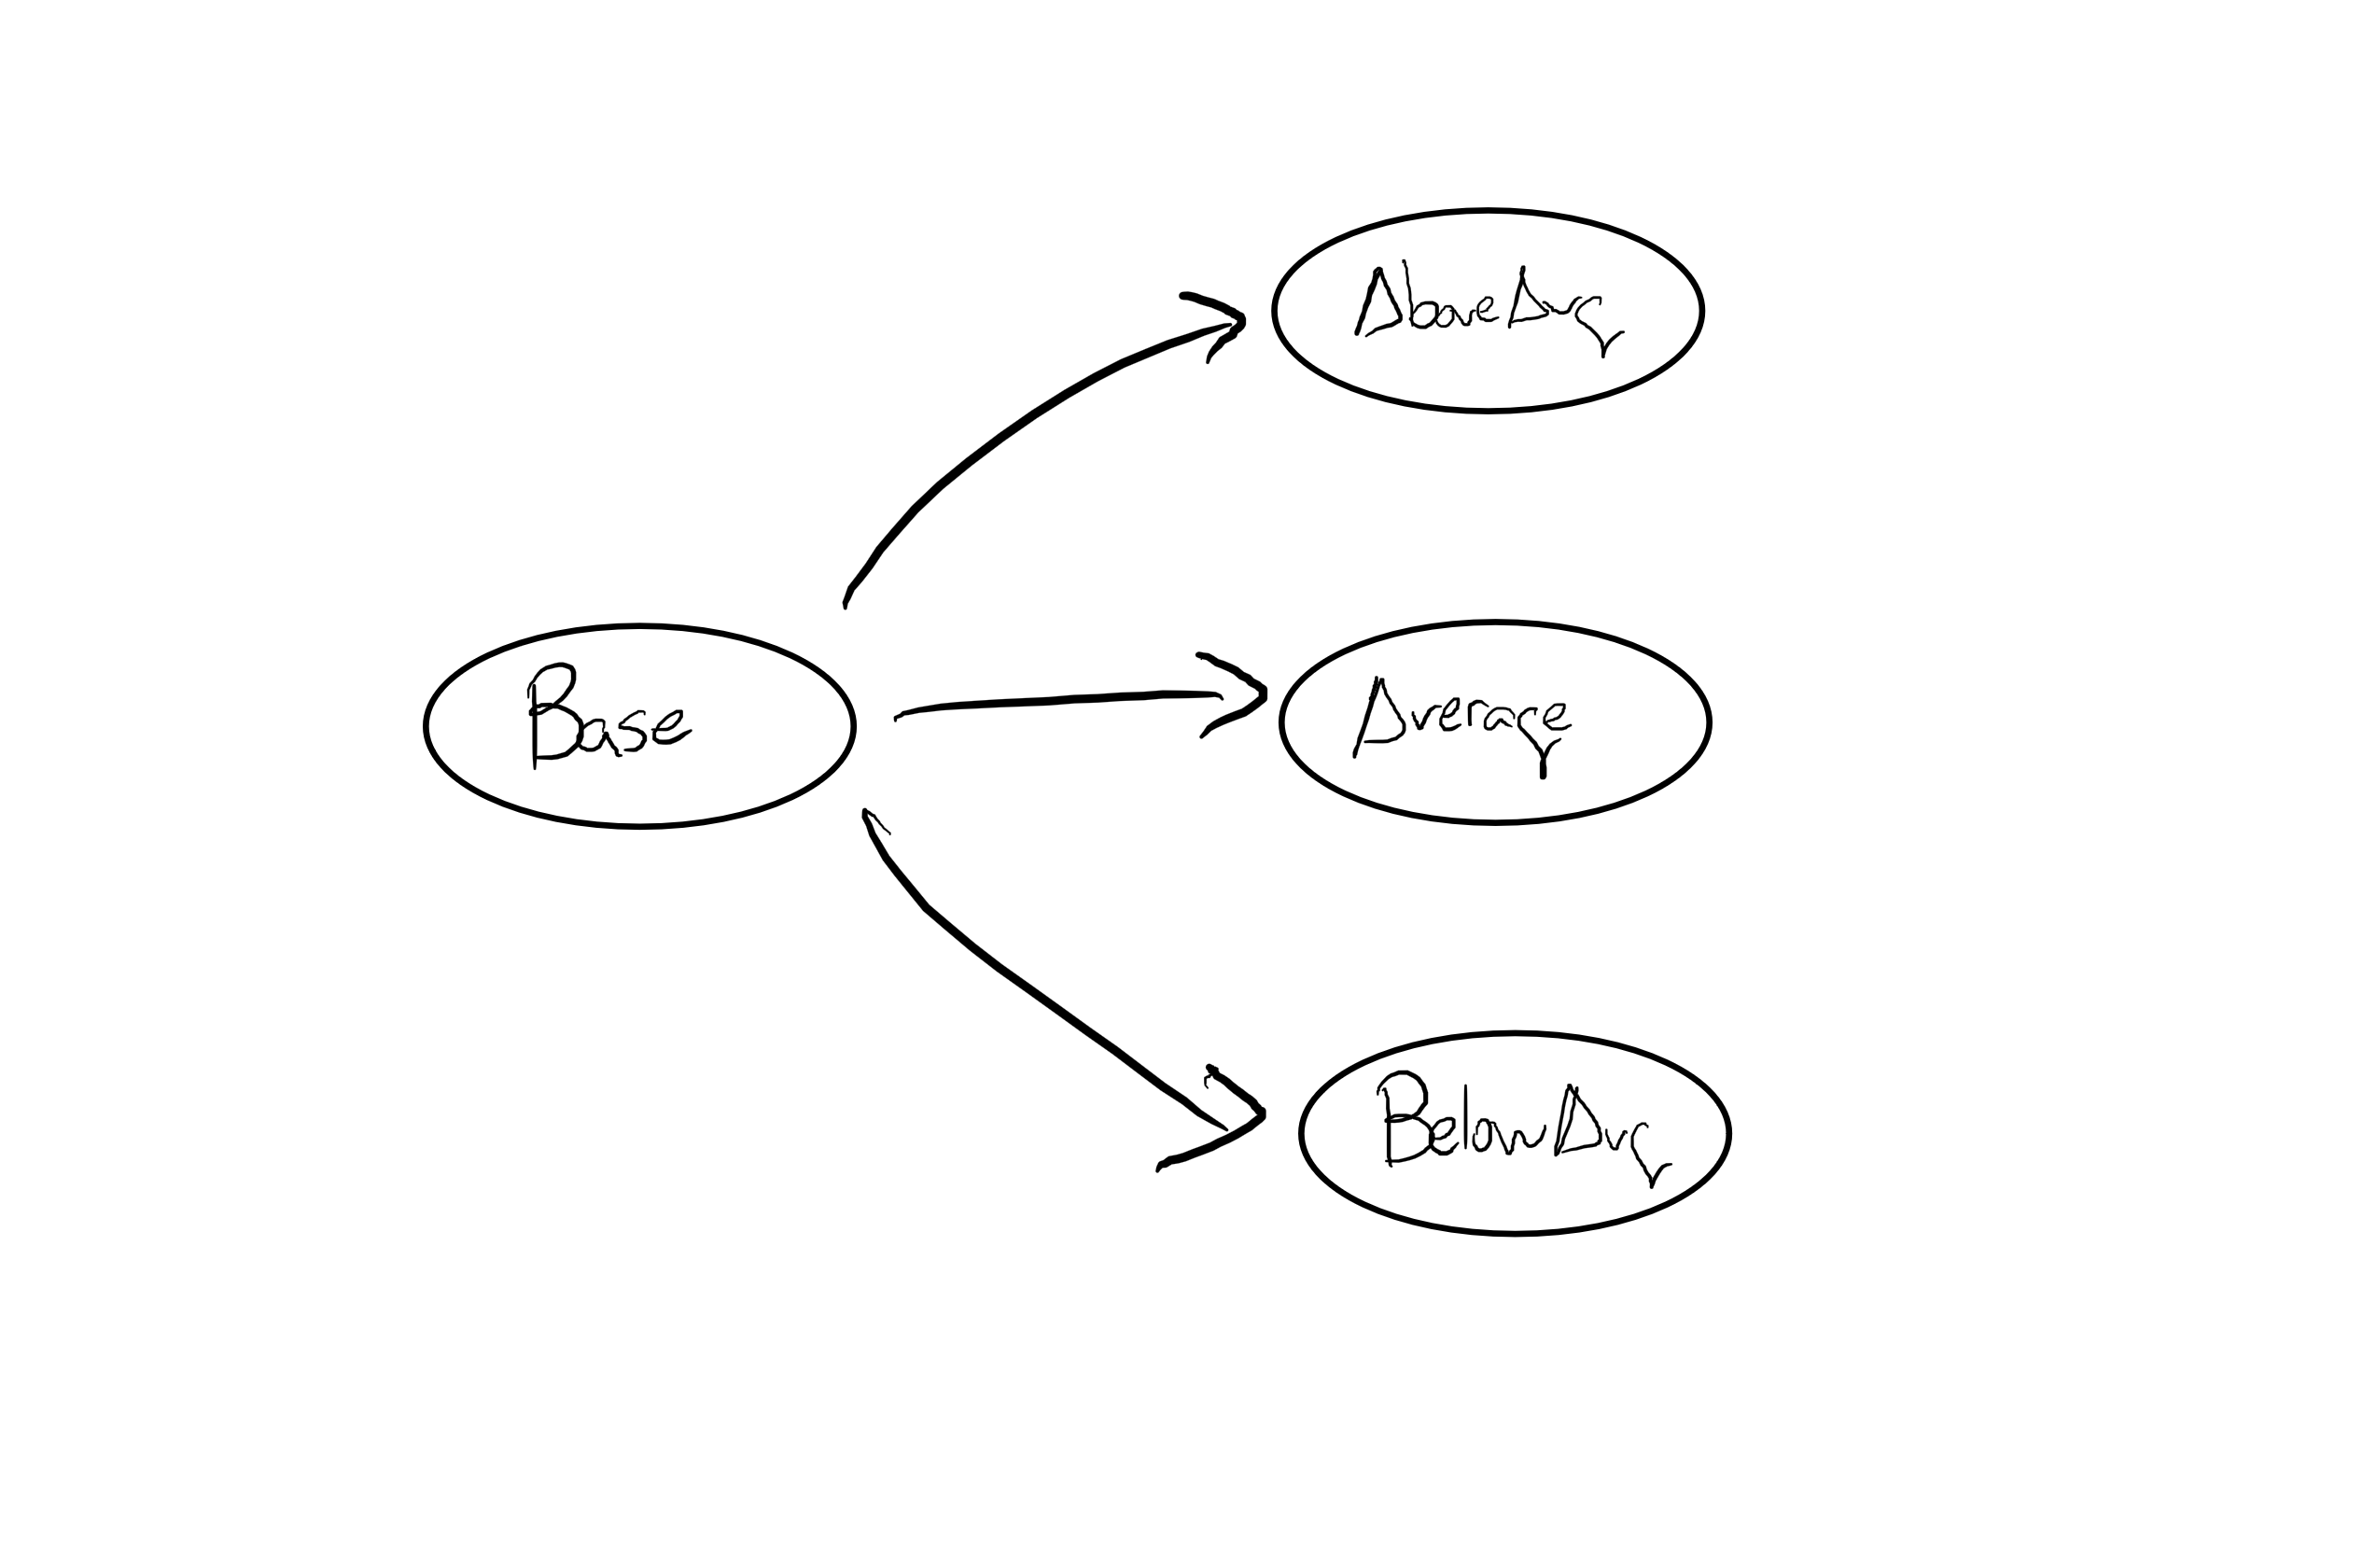
\includegraphics[width=15cm]{figuras/scenario-tree.png}}
    \caption{Árbol de escenarios en un problema estocástico}
\end{figure}

Este tipo de problemas es muy común en el mundo real. Por ejemplo, en una tesis para la Universidad de Chile \cite{thesisHydro}, se utiliza la programación estocástica aplicada a la coordinación hidrotérmica. Este problema ``busca encontrar la operación óptima para un Sistema Eléctrico Mixto, combinando en la solución los efectos de las etapas futuras así como los efectos que la hidrología tiene en la operación del sistema''. Es un problema de optimización para una red energética gubernamental donde se deben tener en cuenta costes y eficiencia de cada tipo de generación de energía, además de contar con factores externos. \\

Los problemas estocásticos pueden subdividirse en problemas individuales (un problema para cada combinación de posibles escenarios generados) lo que los hace un claro objetivo de paralelización. Estos problemas individuales deben converger a una solución única, lo que se consigue con un algoritmo como el \textit{Progressive Hedging} el cual hace uso de las variables concretas de cada escenario y el valor de control $\rho$ para hacer converger las soluciones a un valor equivalente a la resolución del problema antes de subdividirlo.

\section{Motivación del proyecto}

% Adaptarse a nuevas tecnologías para abarcar problemas de mayor tamaño.

Como se ha explicado en el apartado anterior, los problemas estocásticos representan situaciones comunes y su solución puede ser aplicable a muchos campos diferentes. Además, Pyomo ya dispone de herramientas para solucionar este tipo de problemas de forma sencilla, siendo incluso posible hacerlo de forma paralela.\\

Este proyecto tiene como objetivo realizar una nueva implementación alternativa haciendo uso de herramientas Big Data como Spark o tecnologías como MPI. Esta implementación funcionará como base para la resolución de problemas estocásticos en entornos distribuidos, siendo susceptible de recibir optimizaciones concretas para la tecnología escogida y plataformas futuras.

\section{Estado del arte}

% Hablar de Big Data, su orientación principal al manejo de datos masivo. Haremos una adaptación a usarlo como motor de cálculo en entornos de computación distribuida.

Existen múltiples métodos para solucionar problemas estocásticos. Una forma es solucionar la ``representación extendida'' del problema. En este caso se preprocesa el árbol de escenarios para resolverlo como un problema único.\\

El método en el que se centrará este proyecto es el algoritmo ``Progressive Hedging'' que, como se explicó anteriormente, consiste en la solución de subproblemas y la convergencia de sus soluciones. Podemos ver el algoritmo concreto en \autoref{fig:ph_pseudocode}.\\

\begin{figure}
    \centerline{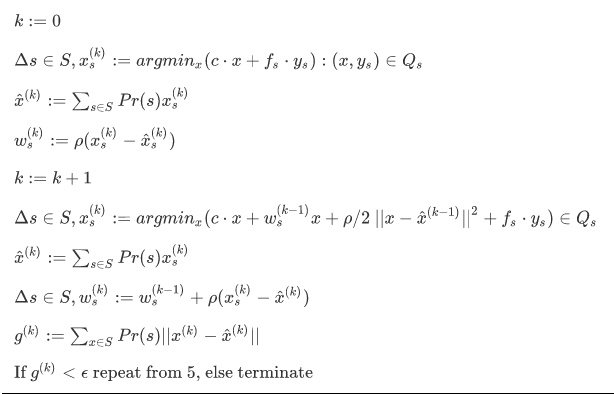
\includegraphics[width=15cm]{figuras/ph-pseudocode.png}}
    \caption{Pseudocódigo del algoritmo Progressive Hedging}
    \label{fig:ph_pseudocode}
\end{figure}

A continuación se especifican las posibles herramientas para implementar este algoritmo y Pyro, la librería utilizada en la implementación paralela ya existente en Pyomo.

\subsection{Big Data}

El término Big Data se refiere al manejo masivo de datos cada vez más relevante en los últimos años. El software orientado a Big Data está optimizado para la obtención, almacenamiento y procesamiento de grandes cantidades de datos que sería inviable analizar con software tradicional. \\

Estudiaremos la herramienta Spark de Apache para la implementación del algoritmo. Spark es un framework de código abierto para la programación en entornos distribuidos. Proporciona una capa de abstracción que permite ejecutar trabajos de forma distribuida sin tener conocimiento de las características del cluster. Spark se encarga de la distribución de los datos, el mantenimiento de su consistencia y la optimización de la repartición.\\

\subsection{MPI}

 MPI, siglas para \textit{``Message Passing Interface''}, es un estándar de paso de mensajes que permite la comunicación entre programas a través de la red. Esta interfaz puede utilizarse para implementar una red de objetos distribuidos y solucionar problemas de forma paralela.\\

 MPI permite el paso de mensajes utilizando tipos primitivos o la creación de tipos personalizados. La comunicación puede ser punto a punto entre dos objetos, sincronizando las llamadas a \textit{send} y \textit{receive}, o puede ser colectiva. MPI también provee funciones para facilitar la ejecución de algoritmos distribuidos como MPI\_BCAST, MPI\_SCATTER o MPI\_REDUCE.
 
\subsection{Pyro}

La intención de este proyecto es realizar una implementación paralela del algoritmo progressive hedging. Para cumplir este objetivo satisfactoriamente, debemos fijarnos en la implementación existente que, en este caso, utiliza la librería Pyro \cite{pyro}. \\

Pyro es una librería de Python para la implementación de objetos remotos. Funciona de una forma similar a RMI de Java, utilizando un servidor de nombres donde los objetos son registrados. Una vez hecho el lookup de un objeto remoto se puede utilizar como un objeto nativo de python, pero la ejecución se realizará sobre el objeto remoto.\\

Este tipo de comunicación entre objetos permite adaptar de forma sencilla un algoritmo implementado con una arquitectura basada en objetos a un entorno paralelo. Sin embargo, este tipo de comunicación tiene ciertas desventajas:

\begin{itemize}
    \item Se debe gestionar manualmente la repartición de trabajo en un entorno distribuido.
    \item No es sencillo optimizar la distribución de memoria entre los nodos de trabajo.
\end{itemize}

\section{Objetivos}

% Los objetivos expuestos en el anteproyecto: generar un módulo para Pyomo y evaluar su rendimiento.

El objetivo principal de este trabajo es paralelizar el algoritmo Progressive Hedging del módulo PySP. Este objetivo principal puede subdividirse en los siguientes objetivos específicos:

\begin{itemize}
    \item Estudiar y analizar el funcionamiento del algoritmo Progressive Hedging en PySP.
    \item Análisis de las diferentes alternativas de paralelización disponibles que mejor se adapten al problema. Se tendrán en cuenta tecnologías Big Data (Apache Spark) o modelos tradicionales (MPI).
    \item Diseño e implementación del nuevo módulo e integración con Pyomo.
    \item Análisis y evaluación del rendimiento.
\end{itemize}

\section{Estructura de la Memoria}

% Lista con los capítulos y qué se trata en cada uno de ellos.

En los siguientes apartados de este documento se especificará el desarrollo del proyecto necesario para el cumplimiento de los objetivos anteriores.

\begin{itemize}
    \item \textbf{\autoref{sec:gestion}: } Especifica aspectos relativos a la gestión del proyecto indicando alcance, requisitos, riesgos, costes y el cronograma del proyecto.
    \item \textbf{\autoref{sec:pruebas}: } Determina las pruebas a realizar sobre la implementación para establecer un nivel de confianza concreto sobre el funcionamiento del mismo. Adicionalmente, se establecerán medidas de rendimiento de la nueva implementación.
\end{itemize}
\cleardoublepage
\chapter{Gestión del proyecto}
\label{ch:gestion}

\section{Alcance}

\subsection{Descripción del alcance del proyecto}

En este proyecto se construirá un módulo software como parte del proyecto Pyomo. Este nuevo módulo adaptará el funcionamiento del actual módulo de programación estocástica (\textit{PySP}) a una implementación paralela.\\

Se realizará un estudio inicial de Pyomo para decidir la integración y la tecnología a utilizar para la nueva implementación. El objetivo de esta nueva implementación es el de proporcionar una ejecución más escalable que permita abordar problemas de mayor tamaño o, al menos, proporcionar una implementación base que, con futuras optimizaciones, permita conseguir ese objetivo.\\

El rendimiento de esta nueva implementación estará reflejado en un informe tras hacer pruebas con distintos problemas y en distintos sistemas.

\subsection{Criterios de aceptación}

El proyecto será aceptado cuando se superen las pruebas definidas en el \autoref{ch:pruebas}.\\

El proyecto persigue dos objetivos: la implementación del algoritmo en paralelo y un estudio de rendimiento. La nueva implementación debe ser capaz de resolver problemas estocásticos de forma paralela usando el algoritmo \textit{Progressive Hedging} y su rendimiento debe escalar añadiendo nodos de computación. Esta implementación debe poder ejecutarse sobre una instalación remota de Spark y utilizando como entrada los mismos modelos de problema que la versión actual de Pyomo. 

\subsection{Entregables del proyecto}

Los elementos a entregar tras la finalización del proyecto son:

\begin{itemize}
    \item Código de Pyomo actualizado con el módulo de ejecución de PH paralelo.
    \item Estudio de rendimiento (incluído en el documento actual).
    \item Memoria de realización del proyecto.
    \item Otra documentación asociada a la realización del proyecto.
\end{itemize}

\subsection{Exclusiones}

El proyecto producirá una implementación paralela del algoritmo PH existente. Esta implementación debe ser funcional pero no es un objetivo del proyecto hacer que esta nueva implementación sea mejor que la anterior en términos de eficiencia o rapidez.\\

Pyomo permite el uso de plugins externos que se pueden ejecutar antes o después de calcular la solución y pueden modificar la entrada/salida del mismo. No se harán pruebas de compatibilidad de la nueva solución con estos plugins de terceros en Pyomo. Sólo se verificará su funcionamiento con la ejecución incluida por defecto.

\subsection{Restricciones}

El proyecto debe finalizar el día 18/06/2018. En caso de ser necesario se puede postponer la fecha de finalización hasta el 27/07/2018.

\section{Análisis de requisitos}

El objetivo principal de este trabajo es el de paralelizar el algoritmo \textit{Progressive Hedging} del módulo PySP. Para conseguirlo se establecen los siguientes requisitos:

% TODO: Introducción a las tablas y concretar algo más. Introducción similar a lo explicado en la sección de riesgos.
% TODO: Añadir requisitos no funcionales y casos de uso.

\Req [
    id=RF-01,
    name={Ejecución de trabajos en Spark},
    description={Ejecutar el algoritmo PH en Spark de forma paralela.},
    priority={Imprescindible}
] { \caption{RF-01: Ejecución de trabajos en Spark}
    \label{tab:rf01}}

\Req [
    id=RF-02,
    name={Integración con Pyomo},
    description={La solución implementada debe funcionar como parte del programa Pyomo.},
    priority={Imprescindible}
] { \caption{RF-02: Integración con Pyomo}
    \label{tab:rf-02}}

\Req [
    id=RF-03,
    name={Interoperabilidad con funcionalidad previa},
    description={La nueva implementación no debe impedir el correcto funcionamiento de los módulos de Pyomo existentes.},
    priority={Importante}
] { \caption{RF-03: Interoperabilidad con funcionalidad previa}
    \label{tab:rf-03}}

\Req [
    id=RF-04,
    name={Establecer medición de rendimiento de Spark},
    description={Cuantificar la diferencia de rendimiento y escalabilidad de la nueva implementación.},
    priority={Importante}
] { \caption{RF-04: Establecer medición de rendimiento de Spark}
    \label{tab:rf-04}}

\section{Análisis de riesgos}

Para un proyecto del tamaño y duración estimados para este TFG es de vital importancia analizar los posibles riesgos que pueden poner en peligro la satisfactoria finalización del trabajo.\\

A continuación se especifican los potenciales riesgos junto a su probabilidad, impacto y tratamiento.\\

La probabilidad se medirá como:

\begin{itemize}
    \item \textbf{Muy alta:} Probabilidad de ocurrencia superior al 90\%.
    \item \textbf{Alta:} Probabilidad de ocurrencia superior al 70\%.
    \item \textbf{Moderada:} Probabilidad de ocurrencia superior al 40\%.
    \item \textbf{Baja:} Probabilidad de ocurrencia inferior al 40\%.
\end{itemize}

El impacto que tendrá la ocurrencia del riesgo sobre los activos afectados se medirá como:

\begin{itemize}
    \item \textbf{Catastrófico: } Supone la cancelación de tareas, inhabilidad de cumplir la fecha límite o, por último, la cancelación del trabajo.
    \item \textbf{Serio: } Supone modificaciones importantes pero asumibles en la realización de las tareas o el tiempo asignado a las mismas.
    \item \textbf{Tolerable: } La aparición del riesgo causará la necesidad de trabajo extra pero asumible. También puede suponer eliminar tareas o resultados poco importantes.
    \item \textbf{Irrelevante: } Las consecuencias generadas por el riesgo pueden ignorarse sin efectos demasiado negativos.
\end{itemize}

\RiskItem [
    id={R-01},
    name={Mala gestión del tiempo de realización del anteproyecto},
    description={
        Un anteproyecto erróneo puede suponer el rechazo del mismo. En menor medida, una descripción demasiado concreta puede suponer un limitante a la hora de realización del trabajo.
    },
    probability={Moderada},
    impact={Catastrófico},
    affected={Anteproyecto},
    treatment={Prevención -- Generar una lista de elementos necesarios para el anteproyecto, planificarlos temporalmente y cumplir dicha planificación.},
    indicators={No cumplir la planificación.},
    follow={Semanal.}
] { \caption{R-01: Mala gestión del tiempo de realización del anteproyecto}
    \label{tab:r-01}}

\RiskItem [
    id={R-02},
    name={No identificar correctamente los objetivos del trabajo},
    description={
        Unos objetivos poco claros pueden llevar a realizar trabajo innecesario o no realizar trabajo imprescindible. También pueden ocasionar desarrollo más lento por no saber qué hacer a continuación.
    },
    probability={Moderada},
    impact={Serio},
    affected={Anteproyecto, Planificación temporal, Código},
    treatment={Minimización -- Revisión de los objetivos dispuestos en el anteproyecto con el tutor del TFG. Esta revisión se hará con antelación suficiente para realizar cambios si fuesen necesarios.},
    indicators={Redacción poco clara del propósito del trabajo en la realización del anteproyecto.},
    follow={Semanal.}
] { \caption{R-02: No identificar correctamente los objetivos del trabajo}
    \label{tab:r-02}}

\RiskItem [
    id={R-03},
    name={Inhabilidad para ajustar el trabajo a las horas requeridas},
    description={
        La realización de un TFG tiene establecida una cantidad de horas fija. Su incumplimiento debe estar justificado.
    },
    probability={Alta},
    impact={Tolerable},
    affected={Planificación temporal},
    treatment={Minimización -- Se estimará la duración de las tareas al alza. En caso de que la planificación acabé con más horas de las permitidas, se podrá disminuir la duración de las tareas menos importantes.},
    indicators={La planificación suma más horas de las permitidas.},
    follow={Cada vez que se modifique la planificación.}
] { \caption{R-03: Inhabilidad para ajustar el trabajo a las horas requeridas}
    \label{tab:r-03}}

\RiskItem [
    id={R-04},
    name={Memoria final poco concreta},
    description={
        La memoria del proyecto debe representar fielmente el desarrollo del mismo. Si se retrasa demasiado su realización es posible perder detalles relevantes del proyecto.
    },
    probability={Alta},
    impact={Serio},
    affected={Memoria},
    treatment={Minimización -- Se realizarán, semanalmente o cada 15 días, documentos de progreso que especifiquen las tareas realizadas. Con esto se tendrá una documentación informal pero muy actualizada y concreta.},
    indicators={Parte del desarrollo no está especificado en ningún documento de progreso ni en la memoria final.},
    follow={Semanalmente.}
] { \caption{R-04: Memoria final poco concreta}
    \label{tab:r-04}}

\RiskItem [
    id={R-05},
    name={Incumplimiento del cronograma del proyecto},
    description={
        Por errores de código, inexperiencia o una carga de trabajo externa mayor de lo esperada, algunas tareas pueden durar más de lo planificado.
    },
    probability={Muy alta},
    impact={Serio},
    affected={Planificación temporal},
    treatment={Prevención -- Seguir el porcentaje de cumplimiento de las tareas sobre el cronograma.},
    indicators={Una tarea no se finaliza en plazo o el porcentaje de realización no es suficiente para el tiempo establecido en la tarea.},
    follow={Diario.}
] { \caption{R-05: Incumplimiento del cronograma del proyecto}
    \label{tab:r-05}}

\RiskItem [
    id={R-06},
    name={Incompatibilidad de la herramienta escogida con Pyomo},
    description={
        Se hará un estudio de herramientas para paralelizar el algoritmo. Si esta herramienta sufre algún tipo de incompatibilidad con el proyecto existente supondrá un retraso importante.
    },
    probability={Baja},
    impact={Catastrófico},
    affected={Diseño, Código},
    treatment={Prevención -- Durante la elección de la herramienta se harán pruebas sencillas sobre el proyecto. Tras crear el diseño se hará una implementación de prueba.},
    indicators={Aparecen errores en el programa que no son causados por fallos de programación.},
    follow={Semanal durante la fase de diseño. Cada 15 días durante la implementación.}
] { \caption{R-06: Incompatibilidad de la herramienta escogida con Pyomo}
    \label{tab:r-06}}

\RiskItem [
    id={R-07},
    name={Retraso del proyecto},
    description={
        Alguna de las tareas planificadas dura más de lo especificado. El impacto dependerá de la gravedad del retraso.
    },
    probability={Moderada},
    impact={Variable},
    affected={Todos los ECS},
    treatment={Minimización -- La planificación se creará con un margen de retraso proporcional a la complicación de la tarea.},
    indicators={Una tarea está tardando en finalizar más de lo esperado.},
    follow={Semanalmente.}
] { \caption{R-07: Retraso del proyecto}
    \label{tab:r-07}}

\RiskItem [
    id={R-08},
    name={No conseguir acceso a un cluster},
    description={
        Para probar el software es ideal utilizar un cluster de computación que permita evaluar la escalabilidad de la solución.
    },
    probability={Moderada},
    impact={Serio},
    affected={Memoria, Informe de rendimiento},
    treatment={Aceptar -- La pruebas se realizarán en un ordenador personal y es posible que tengan resultados menos relevantes.},
    follow={Al finalizar la implementación y al comenzar la ejecución de las pruebas.}
] { \caption{R-08: No conseguir acceso a un cluster}
    \label{tab:r-08}}

\section{Análisis de costes}

En esta sección se realizará un cálculo de los costes del proyecto basados en la planificación temporal establecida.\\

\subsection{Costes materiales}

En primer lugar se hará un cálculo de los costes materiales necesarios para la realización del proyecto.

El único material utilizado ha sido el ordenador de desarrollo. Considerando una vida útil de 4 años y un precio base de 800{\euro} el precio de su uso a lo largo de 78 días es:

\begin{equation}
    \frac{800}{365*4} * 78 = 42\mbox{\euro}
\end{equation}

Todo el software utilizado para la realización del proyecto es gratuito a excepción de MSProject, del cual se hizo uso de la licencia de prueba gratuita.

\subsection{Costes personales}

El coste del desarrollador se estima en 16.300{\euro} brutos. Deduciendo IRPF y costes de Seguridad social, se estima el coste por hora en 17{\euro}.\\

Se deben tener en cuenta los gastos que suponen las reuniones con el tutor del TFG. Se calcula un coste por hora de 28{\euro} y un tiempo total de reuniones en 25h.\\

Si el proyecto dura 78 días y está planificado para un trabajo diario de 5h, los costes personales son:\\

\begin{tabularx}{\linewidth}{|p{3cm}|X|}
    \hline
    \textbf{Desarrollador} & $17*78*5=6630\mbox{\euro}$ \tabularnewline
    \hline
    \textbf{Tutor} & $28*25=700\mbox{\euro}$ \tabularnewline
    \hline
\end{tabularx}

\subsection{Costes indirectos}

Estos costes no están directamente relacionados con el desarrollo del proyecto pero proveen bienes necesarios para la realización del mismo. Entre ellos se encuentran servicios básicos como electricidad e internet.\\

Durante la realización del proyecto se hace uso de estos servicios proporcionados por la universidad mediante el Servicio Universitario de Residencias. \\

Considerando que el proyecto supone 5h diarias, esto es un 13\% del tiempo de uso de dichos servicios. Por lo tanto, en 5 meses (teniendo en cuenta la realización del anteproyecto): 29,25{\euro}

\subsection{Costes tras la ampliación del proyecto}

Una vez modificada la fecha de finalización del proyecto contamos con un mes adicional de gastos. Este nuevo mes debe contar con nuevos gastos indirectos por residir en la vivienda personal, lo que también implica un coste de 10{\euro} por cada reunión que suponga un desplazamiento a Santiago.\\

Esta nueva fecha de finalización supone 40 días extra de gasto. \\

En cuanto a costes materiales, se sumarán 40 días al uso del ordenador, sumando 22{\euro} extra.\\

Los gastos personales, asumiendo otras 15h extra para el tutor:\\

\begin{table} [H]
    \begin{tabularx}{\linewidth}{|p{3cm}|X|}
        \hline
        \textbf{Desarrollador} & $17*40*5=3400\mbox{\euro}$ \tabularnewline
        \hline
        \textbf{Tutor} & $28*15=420\mbox{\euro}$ \tabularnewline
        \hline
    \end{tabularx}
    \caption{Costes personales del proyecto}
    \label{tab:costes-personales}
\end{table}
\ \\
En los gastos indirectos, el precio ahora es superior, contando 57{\euro} de conexión a internet a mayores del resto de facturas, manteniendo el 13\% de uso, suma otros 90{\euro} en los meses de Junio y Julio.\\

Adicionalmente, se consideran 3 reuniones en este periodo adicional, con un coste de 13{\euro} cada una.

\subsection{Resumen de costes}

\begin{table} [h]
    \begin{tabularx}{\linewidth}{|p{3cm}|X|}
        \hline
        \textbf{Personales} & 10.850{\euro} \tabularnewline
        \hline
        \textbf{Materiales} & 64{\euro} \tabularnewline
        \hline
        \textbf{Indirectos} & 158,25{\euro} \tabularnewline
        \hline
    \end{tabularx}
    \caption{Resumen de costes del proyecto}
    \label{tab:costes-resumen}
\end{table}
    \ \\
De esta forma determinamos un \textbf{coste total del proyecto} de 11.072,25{\euro}

\section{Gestión de la configuración}

Para especificar la Gestión de la Configuración de este proyecto primero debemos identificar los Elementos de Configuración de Software (ECS), es decir, los elementos que se verán afectados por esta Gestión de la Configuración.\\

Elementos de Configuración:
\begin{itemize}
    \item Proyecto de software.
    \item Memoria del proyecto.
    \item Anteproyecto.
    \item Documentos de análisis y diseño.
    \item Informes de progreso.
    \item Plantillas de documentos.
\end{itemize}

Para gestionar las diferentes versiones de estos elementos de configuración se creará un repositorio git alojado en Github. Este repositorio contendrá toda la documentación. Para añadir el proyecto de software se realizará un \textit{fork} del proyecto Pyomo original y se añadirá como un submódulo a nuestro repositorio base. \\

Las modificaciones sobre el software serán individuales por lo que no será necesario considerar técnicas de consistencia en trabajo colaborativo. Para los cambios que se realicen se crea una rama específica sobre el \textit{fork} del proyecto.\\

Para relacionar de forma concreta tareas de la planificación con cambios en el repositorio se utiliza un tablero en la plataforma \textit{Trello}. Estas tareas se reflejan en los informes de progreso del repositorio. Además, funciona como herramienta organizativa.

\section{Planificación temporal}

\subsection{Metodología de desarrollo}

% TODO: Explicar elección de cascada.

\subsection{EDT}

\begin{figure}[H]
    \centerline{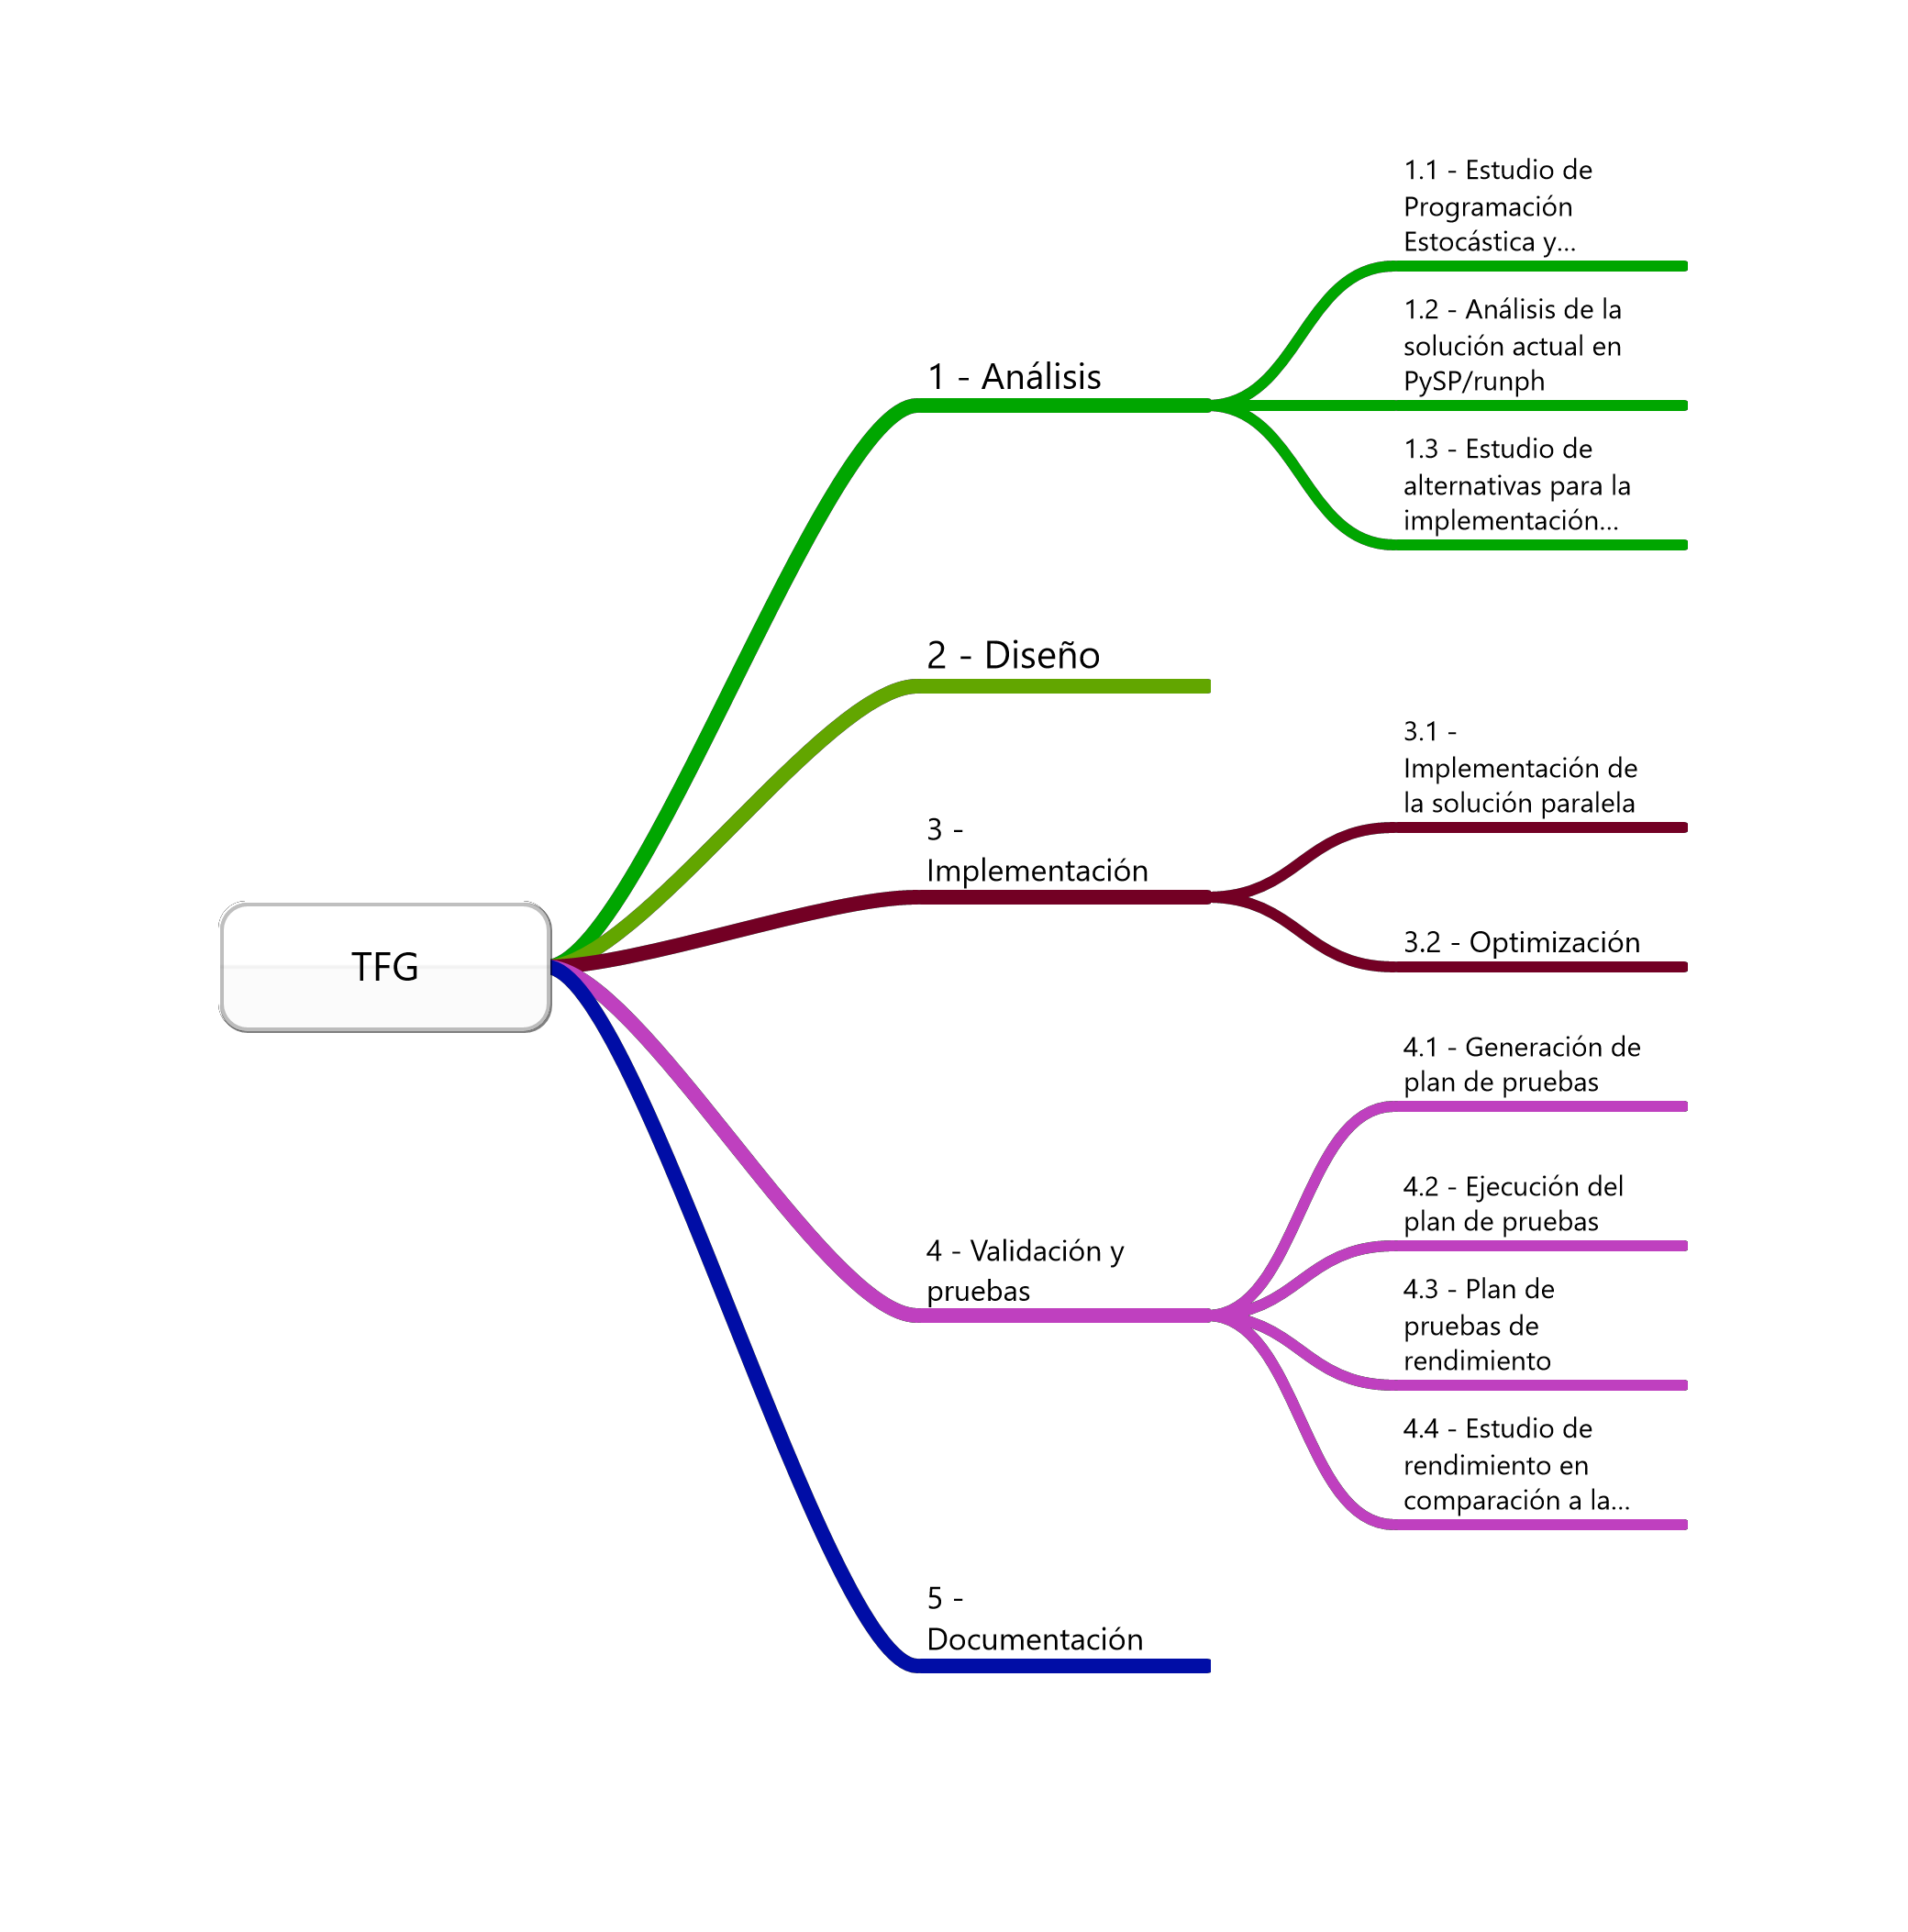
\includegraphics[width=15cm]{figuras/planificacion/edt-inicial.png}}
    \caption{EDT inicial}
\end{figure}

\WorkItem [
            id=1.1, 
            name={Estudio de Programación Estocástica y \textit{Progressive Hedging}},
            description= {
                Se investigará el funcionamiento del algoritmo {\it Progressive Hedging} haciendo uso principalmente de \cite{stochasticProgramming} como referencia.
            },
            duration=7,
            results={N/A}
        ]
{
    \caption{Tarea 1.1: Estudio de Programación Estocástica y \textit{Progressive Hedging}}
    \label{tab:task1.1}
}

\WorkItem [
        id=1.2, 
        name={Análisis de la solución actual en PySP/runph},
        description= {
            Una vez conocido el funcionamiento teórico del algoritmo, estudiar su implementación sobre el proyecto Pyomo.
        },
        duration=8,
        results={Diagrama de funcionamiento PH \cite{local_funcionamientoPH}.}
    ]
{
    \caption{Tarea 1.2: Análisis de la solución actual en PySP/runph}
    \label{tab:task1.2}
}

\WorkItem [
        id=1.3, 
        name={Estudio de alternativas para la implementación paralela},
        description= {
            Se barajarán tecnologías Big Data (Spark) o modelos tradicionales (MPI).
        },
        duration=3,
        results={Resultado del análisis en la \autoref{sec:herramientasAlternativas}}
    ]
{
    \caption{Tarea 1.3: Estudio de alternativas para la implementación paralela}
    \label{tab:task1.3}
}

\WorkItem [
        id=2, 
        name={Diseño},
        description= {
            Generar un diseño de la implementación a realizar con la tecnología escogida. Será importante la integración con la implementación actual.
        },
        duration=20,
        results={Diseño de la implementación.}
    ]
{
    \caption{Tarea 2: Diseño}
    \label{tab:task2}
}

\WorkItem [
        id=3.1, 
        name={Implementación de la solución paralela},
        description= {
            Escribir los nuevos módulos de código e integrarlos en el proyecto. 
        },
        duration=15,
        results={Nuevos ficheros de código y modificaciones a archivos existentes.}
    ]
{
    \caption{Tarea 3.1: Implementación de la solución paralela}
    \label{tab:task3.1}
}

\WorkItem [
        id=3.2, 
        name={Optimización},
        description= {
            Una vez la integración es correcta y la implementación funciona, se realizarán optimizaciones de rendimiento intentando aprovechar las carácterísticas de la tecnología escogida para la nueva implementación paralela.
        },
        duration=5,
        results={Modificaciones a la implementación anterior.}
    ]
{
    \caption{Tarea 3.2: Optimización}
    \label{tab:task3.2}   
}

\WorkItem [
        id=4.1, 
        name={Generación de plan de pruebas},
        description= {
            Idear un plan de pruebas para el nuevo módulo.
        },
        duration=4,
        results={Documento de pruebas \cite{local_planPruebas}.}
    ]
{
    \caption{Tarea 4.1: Generación de plan de pruebas}
    \label{tab:task4.1}
}

\WorkItem [
        id=4.2, 
        name={Ejecución del plan de pruebas},
        description= {
            Implementar y ejecutar las pruebas establecidas para establecer confianza sobre el correcto funcionamiento de la implementación.
        },
        duration=1,
        results={Informe de ejecución de pruebas.}
    ]
{
    \caption{Tarea 4.2: Ejecución del plan de pruebas}
    \label{tab:task4.2}
}

\WorkItem [
        id=4.3, 
        name={Plan de pruebas de rendimiento},
        description= {
            Idear un plan de pruebas con problemas que permitan estudiar el rendimiento del programa.  
        },
        duration=3,
        results={Documento de pruebas de rendimiento \cite{local_planPruebasRendimiento}.}
    ]
{
    \caption{Tarea 4.3: Plan de pruebas de rendimiento}
    \label{tab:task4.3}
}

\WorkItem [
        id=4.4, 
        name={Estudio de rendimiento},
        description= {
            Ejecutar el plan de pruebas anterior y compararlo con las versiones originales tanto secuencial como con Pyro.
        },
        duration=2,
        results={Informe de rendimiento \cite{local_informeRendimiento}.}
    ]
{
    \caption{Tarea 4.4: Estudio de rendimiento}
    \label{tab:task4.4}
}

\WorkItem [
        id=5, 
        name={Documentación},
        description= {
            Generar los documentos asociados al desarrollo del proyecto.
        },
        duration=10,
        results={Memoria del proyecto y documentos asociados.}
    ]
{
    \caption{Tarea 5: Documentación}
    \label{tab:task5}
}

\subsubsection{Tareas no planificadas}

Tras las modificaciones realizadas sobre el cronograma y explicadas en \autoref{sec:modificacionesCronograma}, se generan nuevas tareas para el proyecto: 
 
\WorkItem [ 
        id=3.*,  
        name={Prototipo aislado}, 
        duration=10, 
        description= {
            Crear una aplicación en Python que interactúe con Spark de forma similar a como lo hará la implementación en Pyomo. 
        }
    ] 
{ 
   \caption{Tarea 3.*: Prototipo aislado}
   \label{tab:task.3.*1}
} 
 
\WorkItem [ 
        id=3.*,  
        name={Prototipo de integración inicial}, 
        description= {
            Comenzar la implementación sobre Pyomo comprobando que la integración del nuevo módulo con el código existente es correcta y el flujo de ejecución es correcto con respecto al funcionamiento anterior. 
        },
        duration=5, 
        results={Código añadido a Pyomo.} 
    ] 
{ 
    \caption{Tarea 3.*: Prototipo de integración inicial}
    \label{tab:task3.*2}
} 
 
\WorkItem [ 
        id=3.*,  
        name={Prototipo funcional}, 
        description= {
            Modificar el prototipo anterior añadiendo las funcionalidades esperadas del programa.
        },
        duration=10, 
        results={Código añadido a Pyomo.} 
    ] 
{ 
     \caption{Tarea 3.*: Prototipo funcional}
     \label{tab:task3.*3}
} 

\subsection{Cronograma inicial}

Para la realización del trabajo se plantea un ciclo de vida en cascada. Este ciclo de vida nos permitirá realizar un seguimiento del progreso del proyecto en función del tiempo disponible.

\begin{figure}[H]
    \centerline{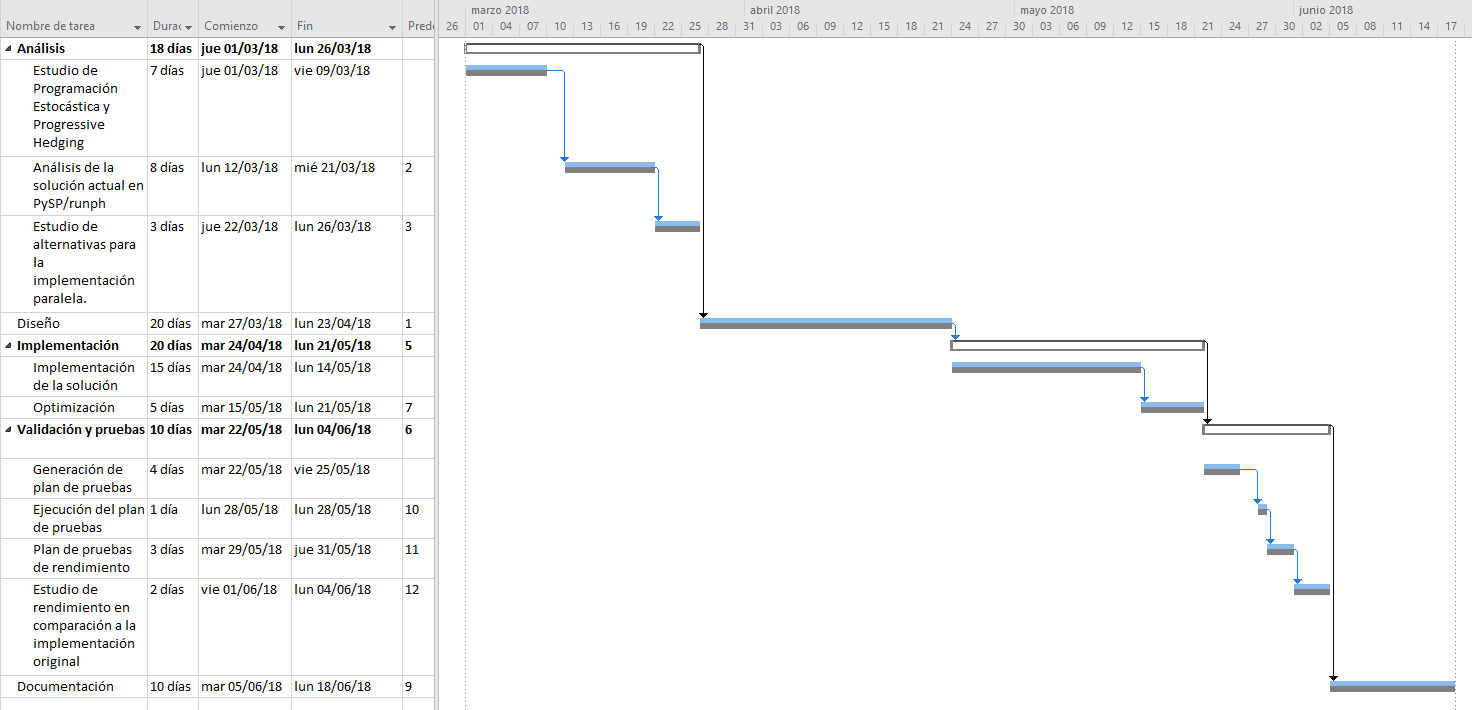
\includegraphics[width=18cm]{figuras/planificacion/linea-base.png}}
    \caption{Línea base}
\end{figure}

\subsection{Modificaciones al cronograma inicial}
\label{sec:modificacionesCronograma}

Se ha realizado una estimación temporal inicial poco precisa por no utilizar ningún tipo de método probado ni datos concretos.

Esta es la razón principal para los retrasos que se explican a continuación.

\subsubsection{Retraso en análisis}

El primer retraso se produce en la fase de análisis de la implementación actual. En esta fase se debe estudiar el funcionamiento del proyecto Pyomo y, en concreto, el módulo de resolución de problemas mediante \textit{Progressive Hedging}. 

A pesar de conocer el funcionamiento teórico del algoritmo mediante \cite{progressiveHedging}, Pyomo es un proyecto complejo, con multitud de funcionalidades para resolver otros tipos de problemas, soporte para plugins, etc. Todo esto hace que la complejidad del código aumente y sea necesario estudiar múltiples capas de abstracción para entender correctamente el funcionamiento del programa.

Otra complicación añadida es el personal desconocimiento del lenguaje Python previo a la realización de este trabajo.\\

Tras este primer retraso se intenta ajustar la planificación reduciendo el tiempo de diseño a la mitad:

\begin{figure}[H]
    \centerline{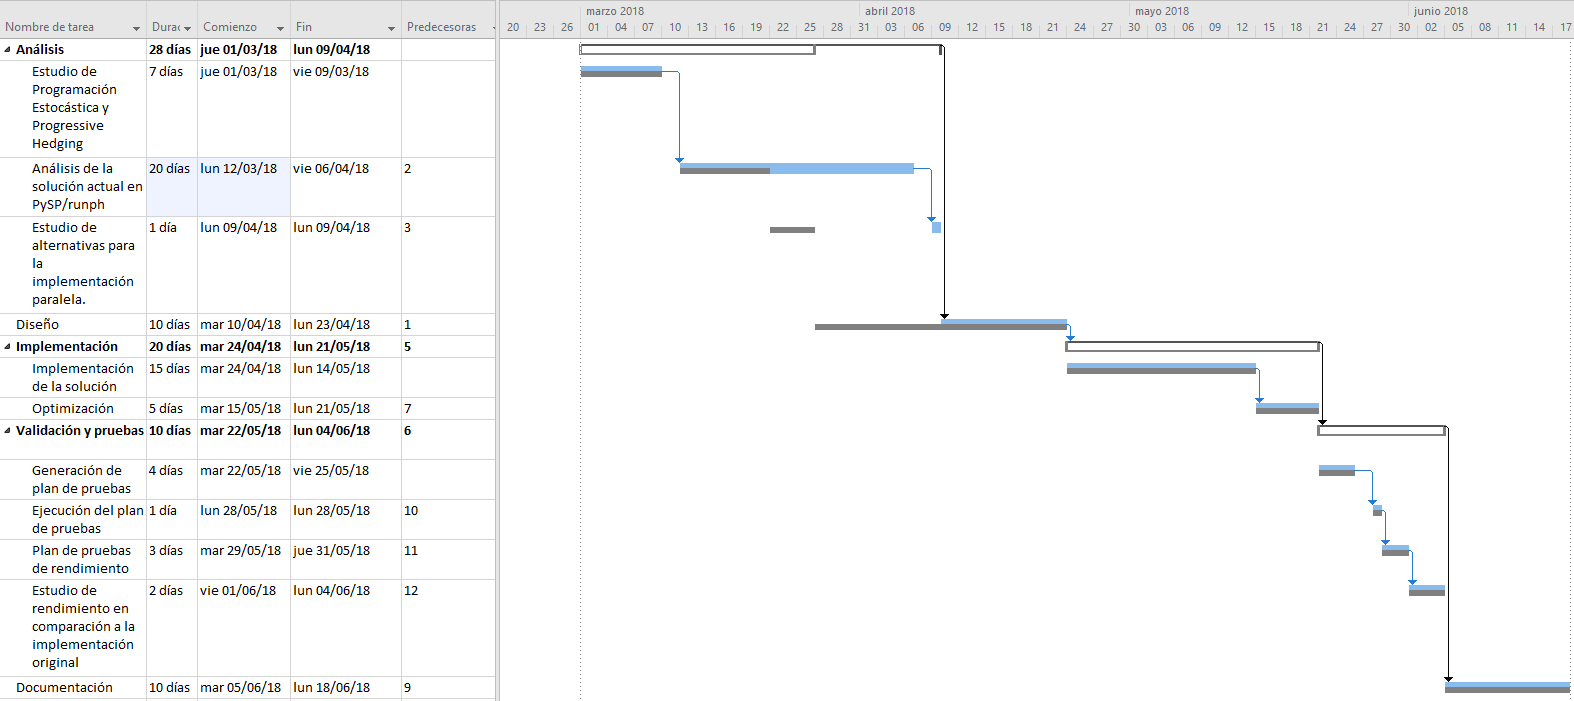
\includegraphics[width=18cm]{figuras/planificacion/1_retraso-analisis-inicial.png}}
    \caption{Primer retraso}
\end{figure}

Teniendo en cuenta que los primeros retrasos fueron principalmente causados por el desconocimiento de la tecnología a usar así como de una mala estimación, es muy probable que en las fases siguientes se produzcan otros retrasos. En este punto se considera entonces abandonar el ciclo de vida en cascada. Su principal atractivo era poder ajustarnos a una planificación temporal que nos permita acabar el proyecto dentro de tiempo, pero esta ventaja no se está cumpliendo en la práctica. Buscando reducir el tiempo de implementación con tecnologías que serán usadas por primera vez, se decide adaptar la planificación a un ciclo de vida por prototipos. 

La creación de sucesivos prototipos permite ir acostumbrándose a las tecnologías desconocidas, en este caso Python y Spark, así como ir probando el rendimiento y la integración a medida que se desarrolla.

En primer lugar se crea un prototipo aislado para comprobar la implementación de Spark con una arquitectura similar a la que se implementará en Pyomo. Este primer prototipo sirve como aprendizaje de la instalación de Spark y el despliegue de una aplicación en el mismo, así como la implementación en Python que interactuará con Spark. Es deseable utilizar una arquitectura de objetos Python similar a la que se usará en Pyomo para concretar el uso de Spark y descubrir posibles problemas con la implementación elegida.

Posteriormente se realizarán prototipos sucesivos sobre Pyomo para integrar el nuevo módulo e ir solucionando posibles problemas de rendimiento o funcionamiento que vayan surgiendo. 

Dado que la implementación partirá de un protipo inicial de baja calidad será importante realizar una fase de optimización y refactorización al final de la implementación para asegurarse un código final de calidad. Definir la calidad del código no es algo trivial y en este caso calificaremos el código como "de calidad" si cumple:

\begin{itemize}
    \item Funciona correctamente y es resistente a errores. Para esto nos apoyaremos en un plan de pruebas funcional.
    \item Funciona eficientemente y otorga un buen rendimiento, en comparación a las implementaciones existentes. En este caso nos apoyaremos en el plan de pruebas de rendimiento.
    \item Se integra adecuadamente al proyecto actual. Debe seguir una filosofía de diseño análoga al resto del código así como funcionar correctamente de forma paralela a todo lo implementado previamente.
\end{itemize}

Tras esta modificación en la planificación, se genera una nueva planificación que podemos ver en la figura y se guardará como una nueva línea base.

\begin{figure}[H]
    \centerline{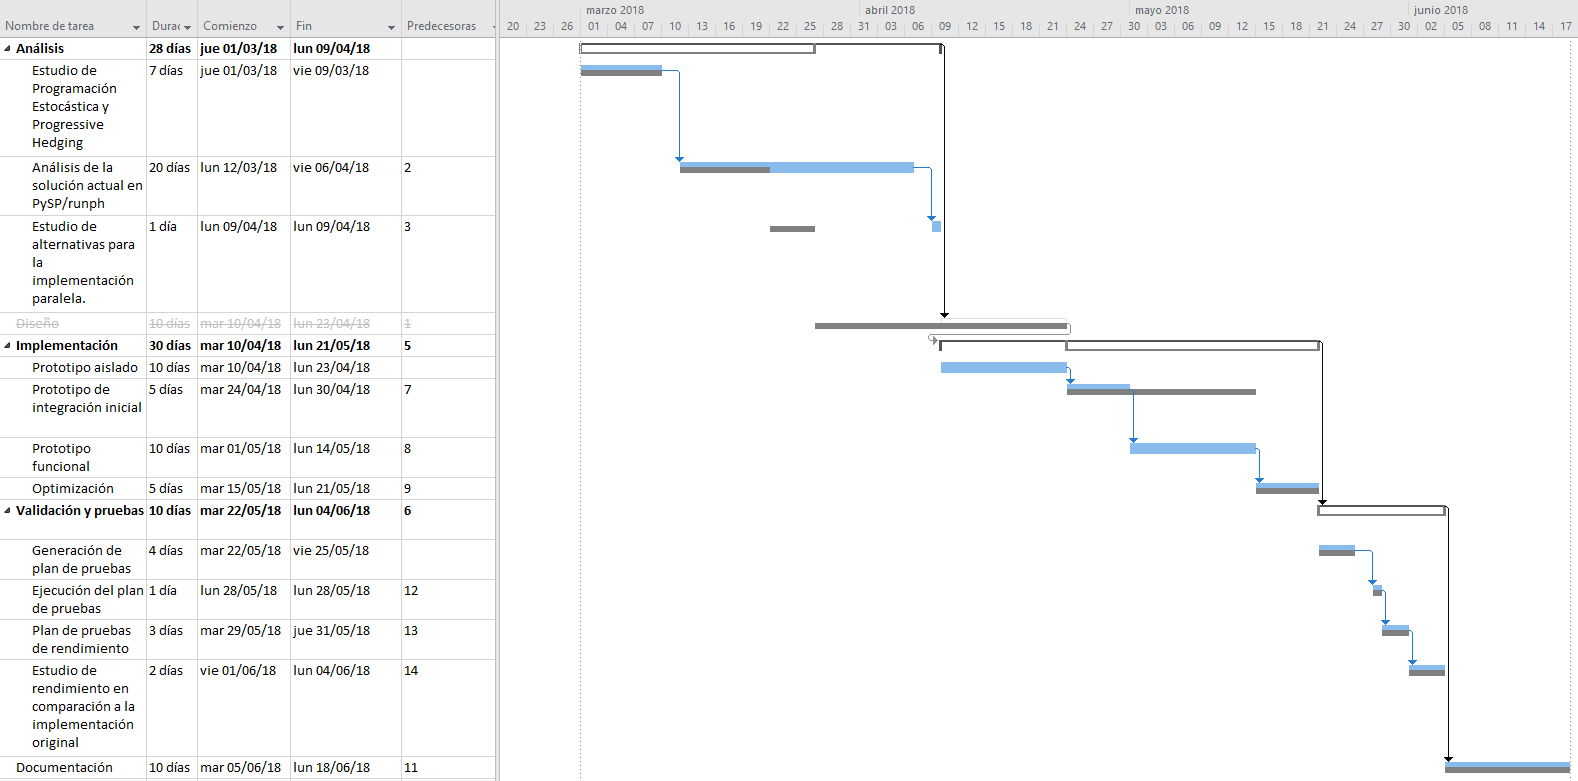
\includegraphics[width=18cm]{figuras/planificacion/2_linea-base-prototipos.png}}
    \caption{Línea base prototipos}
\end{figure}

En este punto hemos eliminado la fase de Diseño para poder aumentar el tiempo asignado a Análisis e Implementación. En caso de sufrir más retrasos en la fase de implementación podremos reducir el tiempo asignado a pruebas si el retraso no es grave. En caso de ser un retraso mayor, no cumpliremos la fecha de finalización establecida.

\subsubsection{Retraso en implementación}

Durante la implementación del prototipo funcional el desarrollo llega a un punto muerto. Las funciones implementadas no devuelven el resultado correcto y se debe hacer una búsqueda de los errores que lo causan. Por falta de experiencia y desconocimiento de las tecnologías, esta fase de implementación se alarga hasta el día 07/07/2018. \\

Este retraso sumado a un retraso de 10 días en la creación del prototipo aislado nos fuerza a retrasar la fecha de finalización del proyecto al día 25/07/2018. \\

Con estos nuevos cambios es necesaria una nueva planificación temporal:

\begin{figure}[H]
    \centerline{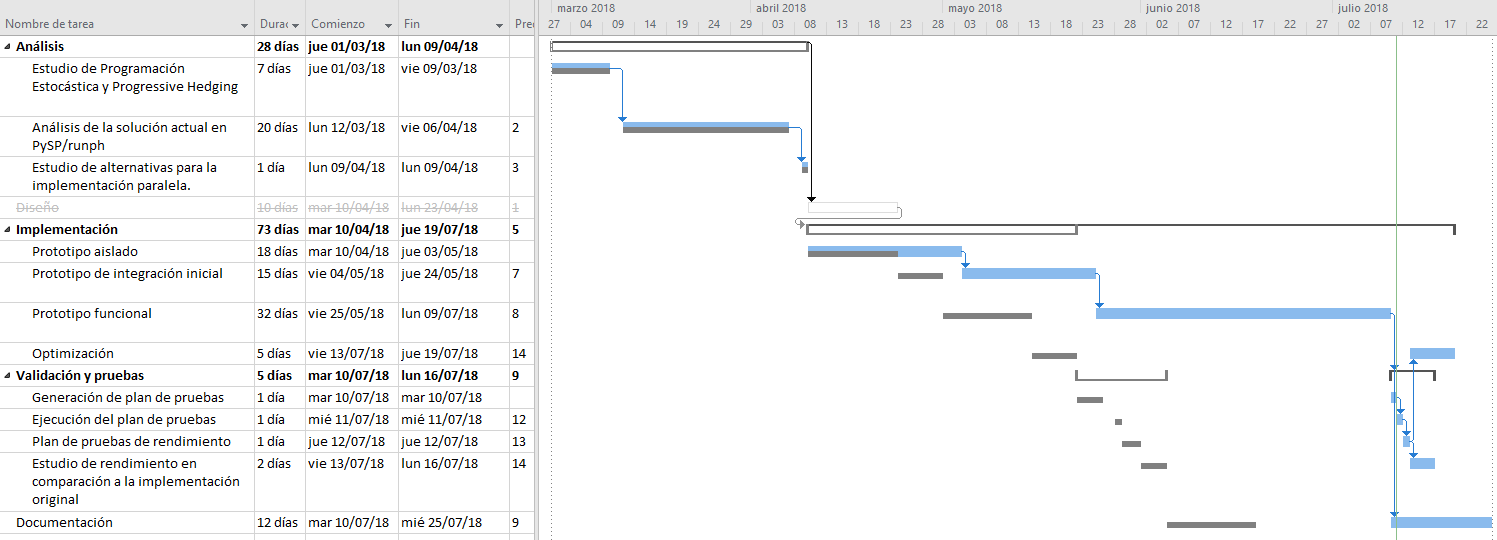
\includegraphics[width=18cm]{figuras/planificacion/3_linea-base-final.png}}
    \caption{Línea base final}
\end{figure}


\cleardoublepage
\chapter{Planificación e presupostos}

Planificación e presupostos: debe incluír a estimación do costo (presuposto) e dos 
recursos necesarios para efectuar a implantación do Traballo, xunto coa planificación 
temporal do mesmo e a división en fases e tarefas. Recoméndase diferenciar os costos relativos a persoal dos relativos a outros gastos como instalacións e equipos.

\cleardoublepage
\chapter{Especificación de requisitos}

Especificación de requisitos: debe indicarse, polo miúdo, a especificación do 
Sistema, xunto coa información que este debe almacenar e as interfaces con outros 
Sistemas, sexan hardware ou software, e outros requisitos (rendemento, seguridade, 
etc).

\cleardoublepage
\chapter{Deseño}

Deseño: cómo se realiza o Sistema, a división deste en diferentes compoñentes e a comunicación entre eles. Así mesmo, determinarase o equipamento hardware e software necesario, xustificando a súa elección no caso de que non fora un requisito previo. Debe achegarse a un nivel suficiente de detalle que permita comprender a totalidade da estrutura do produto desenvolvido, utilizando no  posible representacións gráficas.

\cleardoublepage
\chapter{Exemplos}

\section{Un exemplo de sección}
Esta é {\it letra cursiva}, esta é {\bf letra negrilla}, esta é \underline{letra subrallada}, e esta é {\tt letra curier}. Letra {\tiny tiny}, {\scriptsize scriptsize}, {\small small}, {\large large}, {\Large Large}, {\LARGE LARGE} e moitas más. Exemplo de fórmula: $a=\int_o^\infty f(t)dt$.  E agora unha ecuación aparte:

\begin{equation}
S=\sum_{i=0}^{N-1} a_i^2 .
\label{mi_ecuacion}
\end{equation}

As ecuaciones se poden referenciar: ecuación (\ref{mi_ecuacion}).

\subsection{Un exemplo de subsección}
O texto vai aquí.
\subsection{Otro exemplo de subsección}
O texto vai aquí.
\subsubsection{Un exemplo de subsubsección}
O texto vai aquí.
\subsubsection{Un exemplo de subsubsección}
O texto vai aquí.
\subsubsection{Un exemplo de subsubsección}
O texto vai aquí.
\section{Exemplos de figuras e cadros}

A figura número \ref{enlace1}.

O cadro (taboa) número \ref{enlace2}.

\begin{figure}
\centerline{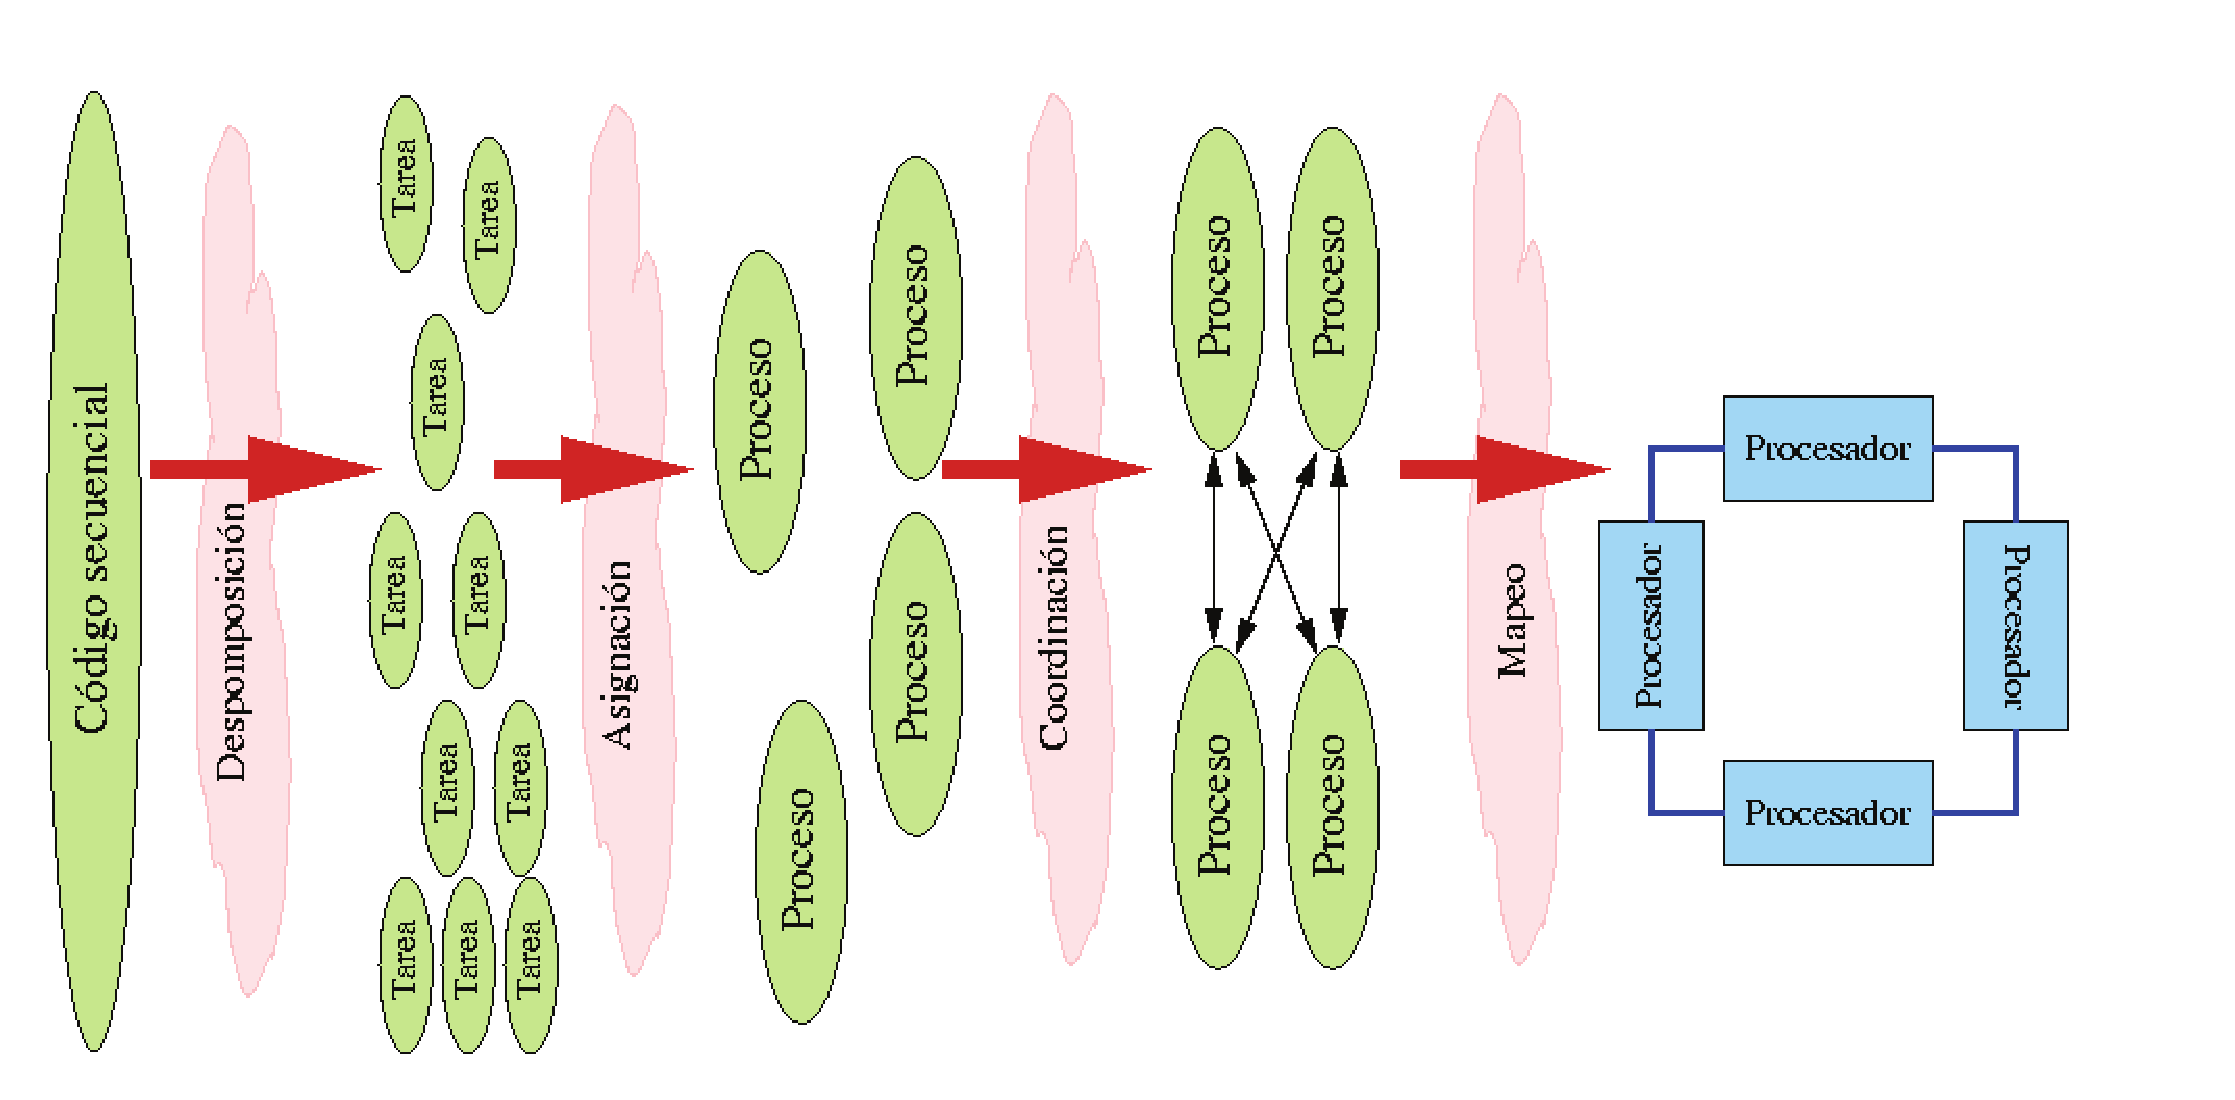
\includegraphics[width=15cm]{figuras/figura01.eps}}
\caption{Esta é a figura de tal e cal.}
\label{enlace1}
\end{figure}

\begin{table}
\begin{center}
\begin{tabular}{|l||r|c|} \hline
Izquierda & Derecha & Centrado  \\ \hline\hline
ll & r & cccc \\ \hline
llll & rrr & c \\ \hline
\end{tabular}
\caption{Esta é a táboa de tal e cal.}
\label{enlace2}
\end{center}
\end{table}

\section{Exemplos de referencias á bibliografía}
Este é un exemplo de referencia a un documento descargado da web \cite{cuda}. E este é un exemplo de referencia a unha páxina da wikipedia \cite{cdma}. Agora un libro \cite{gonzalez} e agora unha referencia a un artigo dunha revista \cite{patricia}. Tamén se poden pór varias referencias á vez \cite{cuda,gonzalez}.

\section{Exemplos de enumeracións}

Con puntos:

\begin{itemize}
\item Un.
\item Dous.
\item Tres.
\end{itemize}

Con números:

\begin{enumerate}
\item Catro.
\item Cinco.
\item Seis.
\end{enumerate}

Exemplo de texto verbatim:

\begin{verbatim}
O texto        verbatim 
     se visualiza tal
            como se escribe
\end{verbatim}

Exemplo de código C:

\lstset{language=C}

\begin{lstlisting}
#include <math.h>
main()
{  int i, j, a[10];
   for(i=0;i<=10;i++) a[i]=i; // comentario 1
   if(a[1]==0) j=1; /* comentario 2 */
   else j=2;
}
\end{lstlisting}

Exemplo de código Java:

\lstset{language=java}

\begin{lstlisting}
class HelloWorldApp {
    public static void main(String[] args) {
        System.out.println("Hello World!"); // Display the string.
    }
}
\end{lstlisting}
%
% Engadir os capitulos que fagan falta
%
\cleardoublepage
\chapter{Conclusións e posibles ampliacións}

Conclusións e posibles ampliacións


% Aquí empezan os apéndices
\appendix
\cleardoublepage
\chapter{Manual de despliegue}

En esta sección se explicará como instalar Spark y ejecutar los ejemplos incluidos en Pyomo con el nuevo módulo \texttt{phspark}.

El primer paso será descargar la distribución de Spark para nuestro sistemas operativo desde la página oficial (\url{http://spark.apache.org/downloads.html}). En el momento de realización de este documento, la última versión es la 2.3.1. Una vez descargado, podemos iniciarlo con la configuración por defecto ejecutando el script \texttt{/sbin/start-all.sh}.

Podemos comprobar que Spark se ha iniciado correctamente accediendo a la interfaz web en \texttt{localhost:8080}, como se ve en la \autoref{fig:manual-spark-web}. En este caso, para acceder al clúster, usaremos la url \texttt{localhost:7077} y esa será la dirección que le indicaremos a Pyomo.\\

\begin{figure}[H]
    \centerline{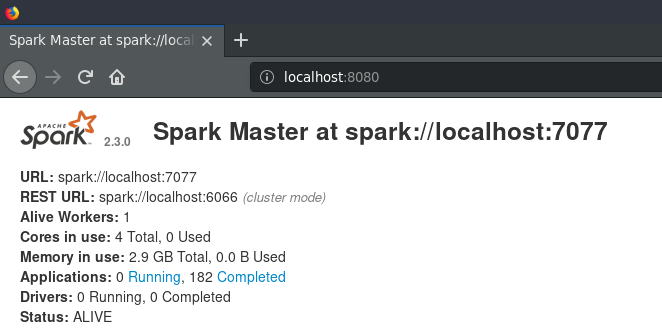
\includegraphics[width=15cm]{figuras/manual/spark-web-interface.png}}
    \caption{Interfaz web de Spark}
    \label{fig:manual-spark-web}
\end{figure}

Teniendo Python 3.6 instalado, vamos a la carpeta raíz del proyecto Pyomo. En esta carpeta hay un archivo \texttt{setup.py}. Para instalar este repositorio de Pyomo como librería en nuestro Python actual, ejecutamos: \\

\texttt{python setup.py develop}. \\

En caso de necesitar librerías adicionales se instalarán usando \texttt{pip}. Algunos requisitos probables son \textit{Pyro} y \textit{Pyutillib}.\\

Con este entorno instalado ya podemos ejecutar los ejemplos de Pyomo utilizando \texttt{phspark}. Para ello, nos movemos a la carpeta \texttt{/pyomo/examples/pysp/farmer} y ejecutamos el siguiente comando:\\

\begin{verbatim}
    runph -r 1 --solver-manager=phspark --traceback --solver=minos
     --solver-io=nl --xhat-method=voting --verbose 
     --model-directory=models/ReferenceModel.py 
     --instance-directory=scenariodata/ScenarioStructure.dat  
     --spark-host=localhost --spark-port=7077
\end{verbatim}

Esto nos mostrará la traza de ejecución y los resultados del problema al final.

\cleardoublepage
\chapter{Manuais de usuario}

Manuais de usuario: incluirán toda a información precisa para aquelas persoas que utilicen o Sistema: instalación, utilización, configuración, mensaxes de erro, etc. A documentación do usuario debe ser autocontida, é dicir, para o seu entendemento o usuario final non debe precisar da lectura de outro manual técnico.

\cleardoublepage
\chapter{Licenza}
Se se quere pór unha licenza (GNU GPL, Creative Commons, etc), o texto da licenza vai aquí.


\cleardoublepage
\markboth{BIBLIOGRAFÍA}{BIBLIOGRAFÍA}
\addcontentsline{toc}{chapter}{Bibliografía}


\begin{thebibliography}{99}
% % EXEMPLO DE DOCUMENTO DESCARGADO DA WEB
% \bibitem{cuda} Nvidia CUDA programming guide. Versión 2.0, 2010. Dispoñible en % {\it http://www.nvidia.com}.
% 
% % EXEMPLO DE PÁXINA DA WIKIPEDIA
% \bibitem{cdma} Acceso múltiple por división de código. Artigo da wikipedia (% {\it http://es.wikipedia.org}). Consultado o 2 de xaneiro do 2010.
% 
% % EXEMEPLO DE LIBRO
% \bibitem{gonzalez} R.C. Gonzalez e R.E. Woods, {\it Digital image processing}, % 3ª edición, Prentice Hall, New York, 2007.
% 
% % EXEMPLO DE ARTIGO DE REVISTA
% \bibitem{patricia} P. González, J.C. Cartex e T.F. Pelas, ``Parallel % computation of wavelet transforms using the lifting scheme'', {\it Journal of % Supercomputing}, vol. 18, no. 4, pp. 141-152, junio 2001.

\bibitem{learningSpark} Matei Zaharia, Patrick Wendell, Andy Konwinski, Holden Karau, {\it Learning Spark: Lightning-Fast Big Data Analysis}, 1ª edición, O'Reilly Media, 2015.

\bibitem{stochasticProgramming} John R. Birge, François Louveaux, {\it Introduction to Stochastic Programming}, 2ª Edición, Springer, 2011.

\bibitem{IEEE829} IEEE Std 829-2008, IEEE Standard for Software and System Test Documentation

% Files local to the project

\bibitem{local_funcionamientoPH} PONER AQUÍ LA RUTA
\bibitem{local_distributedTestApp} Proyecto de pruebas en: ``/DistributedTest''

\end{thebibliography}



\end{document}
